%------------------------------%
\selectlanguage{english}
\chapter{Supporting resource awareness}
\label{chp:background_resource_awareness}
\markboth{Supporting resource awareness}{Chapter1}
%------------------------------%

\coolphrase {Hey, look at this}{Inti Gonzalez-Herrera}

In this chapter, the context of this thesis, the general problem it faces, and the limitations of existent approaches, are introduced.
The ideas behind resource-aware programming are discussed in Section~\ref{sec:resource-awareness},
where the mechanisms required to support resource awareness in a runtime environment are also presented.
Since our work focuses on managed runtime environments, Section~\ref{sec:mrtes} briefly presents the features of this kind of systems that hinder resource-aware programming.
Afterwards, Section~\ref{sec:resource-awareness-related-work} discusses the advantages and limitations of existent solutions to deal with resource consumption monitoring and reservation (two subproblems to tackle to support resource-aware programming).
Finally, this chapter concludes by highlighting the lack of proper support to develop applications that can take advantage of resource awareness, and stating what is needed to improve such support.

\section{Resource-Aware Programming} \label{sec:resource-awareness}

Efficient use of computational resources is an essential concern in software systems because it can reduce the costs of the infrastructure needed to execute applications.
Resource management is nevertheless particularly challenging when many stakeholders share a platform.
As a consequence, a traditional approach for resource management in applications is to rely on the runtime environment (e.g., managing resources is traditionally a main concern of operating systems); and using the environment's generic API to access resources.
Although there are many advantages associated to this approach, it is known that applications built upon such generic interfaces often show relative poor performance \cite{engler1995exokernel}.
The problem arises because the implementation of a general purpose abstraction must cover many use-cases.
This results in complex execution paths where few assumptions regarding how the abstraction will be used can be made.
It has been shown that the performance of many resource intensive systems can be improved by carefully specializing resource management at the application level \cite{engler1995exokernel,Belay:2014:IPD:2685048.2685053,Marinos:2014:NSS:2619239.2626311}.

The principle of bypassing a generic implementation in favor of a specialized one has been widely applied in computer science and software engineering \cite{engler1995exokernel, Munro1996,Dragos:2009:CGT:1565824.1565830,Marinos:2014:NSS:2619239.2626311}.
Since resource usage is a key concern for any software system, specializing resource management is potentially beneficial for many applications.
In this thesis, we use the term \textit{resource-aware} to refer to those applications/systems that observe, carefully manage, and are aware of computational resources in order to improve their performance. 
At first, this definition might look too broad, but in reality most applications limit themselves to carefully use the resource allocations facilities offered by runtime environments.
Take for example a web server that uses a pool of threads to process remote requests.
By using this pool the server is in fact carefully managing resource, but with this feature alone it is not able to observe whether the pool's size should be decreased/increased.
The key issue in the definition used in this thesis is that three elements must be present in an application/system in order to be classified as \textit{resource-aware}: observation, management, and behavior modification.

 
Finally, our understanding of the idea of resource-aware applications/systems is in fact closely related, but not limited, to that of \textit{Autonomic Computing} \cite{Horn2001,kephart03,Brun:2009:ESS:1573856.1573860}.
Figure \ref{fig:resource-aware-vs-autonomic-computing} depicts an example of how the MAPE-K loop can be instantiated to build an autonomic manager that is aware of resource consumption.
During monitoring, two variables are considered: CPU usage and memory availability.
In this abstract example, the analyze phase determines whether some components are misbehaving.
Next, a plan to replace the faulty components is built.
The last step in the loop involves reconfiguring the system to effectively replace the faulty components.
Some knowledge is needed to guide the process; in this case, information on the architecture of the system, its components, and how they are couple, may result beneficial.

\begin{figure}[!h]
\centering
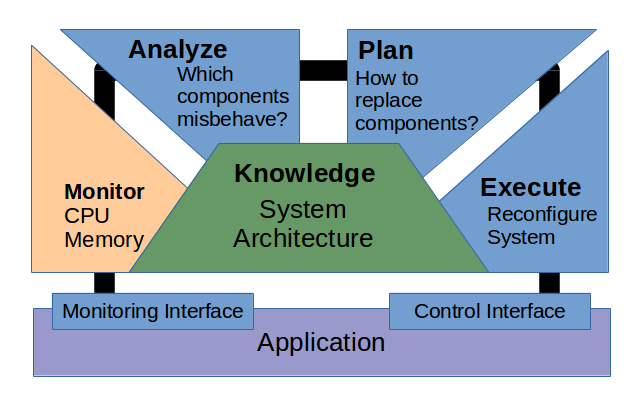
\includegraphics[scale=0.65]{./chapter1/fig/mape-k.png}
\caption{A MAPE-K loop to support system reconfiguration based on resource consumption} \label{fig:resource-aware-vs-autonomic-computing}
%\caption{Resource-aware programming can be seen as a particular case of \textit{autonomic computing.}} \label{fig:resource-aware-vs-autonomic-computing}
\end{figure}

Applying resource-aware techniques to develop a software system can be motivated by the need to satisfy both functional and non-functional requirements.
Among the non-requirements we find the following:

\begin{itemize}
\item \textbf{Improve performance.}
Considerable amount of work showing the potential advantages of specializing resource management to enhance system performance have been published.
Some interesting use-cases are, for instance, reducing the execution time \cite{Polo:2011:RAS:2414338.2414352}, and increasing the number of requests a web server is able to handle \cite{engler1995exokernel,Belay:2014:IPD:2685048.2685053}.

\item \textbf{Guarantee certain Quality of Service (QoS).} 
Often, when the quality of a service is evaluated, we consider properties that are related to either the resources allocated to execute the service or the mechanisms used to manage resources.
For instance, misbehaviors in a property such as response time can be associated to low resource availability \cite{Chechik-2009,autili2012hybrid}.
Likewise, poor QoS in multimedia systems is associated to complex resource management mechanisms in the operating system kernel \cite{Black1997}.
Finally, resource-aware networking can be used to improve QoS properties such as data availability \cite{Boldrini:2008:CRA:1549824.1550106} and P2P video streaming \cite{Pianese:2007:RLA:1326320.1326323,Alhaisoni:2010:RTO:1664767.1664770}.

\item \textbf{Support per-customer resource quotas.}
In Software as a Service (SaaS), it is necessary to guarantee per-tenant quotas.
Although using a new application instance for each tenant is a solution; this approach leads to excessive resource consumption.
On the contrary, one other solution is to design multi-tenant applications - which share most applications' code - by scheduling incoming requests in order to guarantee per-tenant quotas \cite{KrSpAhKo2014_CCGrid_ResourceIsolation,KrWeKo2013-icwe-MTBenchmark}.    

\item \textbf{Ensure resource isolation for critical applications.}
Strong isolation among applications is often required when critical applications \cite{Knight:2002:SCS:581339.581406} share a platform with untrusted software systems.
In this context, resource usage isolation is an important concern because one application can make a second application crash by simply monopolizing the computational resources.
In this scenario, application containment \cite{Kamp00jails:confining,Soltesz:2007:COS:1272998.1273025,Madhavapeddy:2015:JJS:2789770.2789809} is a useful mechanism to support resource-aware isolation.
Providing specialized application containment requires extensive runtime environment support, based on approaches such as \textit{unikernels} \cite{Madhavapeddy:2013:ULO:2499368.2451167, Kivity:2014:OVO:2643634.2643642, Madhavapeddy:2015:JJS:2789770.2789809}, that has been under heavy development after the widespread adoption of distributed and cloud services.  

\end{itemize}

To satisfy these requirements applications often rely on specific features offered by the runtime environment or platform (e.g., operating systems, virtual machines).
In this thesis, three features that result useful to support the resource-aware programming paradigm are identified:

\begin{itemize}
\item \textbf{Resource consumption monitoring.}
Having information regarding how an application is consuming resources is mandatory to support any form of decision making that involves the modification of applications due to resource-related issues. 
In this regard, it is useful to collect data about global application consumption as well as collecting such data for each application's module with clearly defined boundaries (e.g., components).

\item \textbf{Resource reservation.}
Ensuring resource availability for specific applications or subsystems is a way to support critical applications or other systems which exhibit, for instance, timing constrains.
Reserving resources does not always imply that resources must be exclusively assigned to a process.
Instead, for certain resources such as CPU time it is possible to allocate the requested resource once it is needed.

\item \textbf{Observing resource availability (overcommitment).} 
Applications that are aware of extra resource availability are able to temporarily use such resources to improve the QoS they provide.
In addition, applications can nicely modify their behavior to collaborate with other systems that share a platform if they are aware of their consumption, the resource availability and also of what other applications demand.
\end{itemize}

In this research, we focus on two of these features: \textit{resource consumption monitoring} and \textit{resource reservation}.
In particular, this thesis devotes a significant amount of space discussing how to deal with the problem of efficiently monitoring the quantity of resources consumed by different parts of an application.

%\todo{Fill the box}
%\extracomment{Resource-aware vs Real-Time requirments}{
%
%This is an easy way to box text within a document!
%
%czxcvzc. fsfdsfsd.
%}

Providing support for the mentioned features highly depend on the target abstractions provided by the runtime environment.
In an operating systems resource consumption monitoring is often provided at per-process basis while
virtual machine monitors (VMMs) tend to offer per virtual machine resource management.
In this thesis, we focus on offering support for resource-aware programming in managed runtime environments.
Hence, the next section presents a brief overview of the main properties of these systems. 

%Debe resaltarse en un parrafo inicial como todo lo que hace una computadora esta en definitiva asociado con recursos.
%
%Esta seccion describe y define lo que entendemos por resource aware programming. Esto no es muy sencillo puesto que no hay una definion muy formal que digamos.
%
%De hecho, este es un termino al que se hace referencia en varios lugares para referirse a la capacidad de ciertos sistemas de software para adaptar su funconamiento en base ala existencia de recursos.
%
%Es valido destacar en este punto,  la relacion que tiene esto con los sistemas adaptables y reconfigutrables y en defintiva con el concepto general de MAPE Loop.
%
%Ademas, se persiguen objetivos como los siguientes cuando se quiere ser resource aware:
%\begin{itemize}
%\item Mejorar eficiencia
%\item Mejorar parametros de calidad de la aplicacion como availability
%\item Asegurar resource isolation para critical applications
%\item Garantizar cuotas de uso para distintios usuarios
%\end{itemize}
%
%Como lo vemos, hay tres cualidades que pueden pedirse cuando se quiere ser resource aware:
%\begin{itemize}
%\item Resource consumption monitoring
%\item Resource reservation
%\item Observing resource availability (overcommitment) 
%\end{itemize}
%
%
%
%
%Un punto escencial aqui es establecer bien claro cual es la diferencia entre:
%\begin{itemize}
%\item resource awareness vs real-time
%\item resource reservation vs scheduling
%\end{itemize}
%
%El objetivo de esta seccion es dar una fundamentacion clara sobre las motivaciones que guian esta tesis y mostrar los temas en los que estara enfocada.
%
%Es una seccion general que sin embargo tendra citas lo mas actualizadas posible en las secciones cables. La longitud estimada es de 2 a 3 paginas.

\section{Managed Runtime Environments} \label{sec:mrtes}

Applications written using a given programming language often execute in a runtime environment which implements every single built-in feature of the language and supports a specific instruction set.
For a language such as \textit{C++} the runtime environment is in charge, among others, of supporting the \textit{throw/exception} mechanisms and the \textit{type casting} mechanism.
It is common to ship the runtime environment along the application when applications are deployed as native code because external dependencies are avoided in such a way.
However, developers that use mature languages such as \textit{C++} or \textit{Object Pascal} lack useful built-in features that both can ease the development process, and improve applications' quality.

In 1995 the first mainstream managed runtime environment (MRTE), Java, was created. It became a success even if it was not the first language providing built-in features such as automatic memory management, dynamic loading of portable code, or support for the object-oriented paradigm due to three main reasons: the level of maturity of many technical solutions on topics such as just-in time (JIT) compilation, the growing speed-up of hardware, and the advantages offered by the concept of \textit{managed} languages.
Since then, it has become clearer that modern languages demand features which require a considerable runtime support.
These features include the following \cite{Cierniak2005}:

\begin{itemize}
\item \textbf{\textit{Portability}}:
In an ideal scenario, applications should be distributed to customers and deployed in a platform independent format that can be executed on top of specific architectures and platforms.
This helps to reduce the application's time to market.
To provide this feature, the application must be written in such a way that allows its execution on top of an abstract machine which has its own instruction set instead of on top of native platform.
An application can then be executed on a platform if there exists an implementation of this abstract machine that is able to run on such a platform.
Having a different instruction set offers additional advantage.
For instance, final applications' code can be more compact than code written using native instructions because it can represent only the high level concepts that matter to the abstract machine.
To support this feature, a runtime must provide either application's interpretation, ahead of time compilation \cite{Muller:1997:HFE:1268028.1268029,Proebsting:1997:TJA:1268028.1268031,Wang:2011:MAC:2038698.2038704,Oh:2015:BAC:2757012.2757057} or just in time compilation (JIT) \cite{Inoue:2012:AMC:2398857.2384630,Paleczny:2001:JHT:1267847.1267848,Grcevski:2004:JTJ:1267242.1267254}.

\item \textbf{\textit{Dynamic code loading}}:
It is also desirable to support loading new code from different sources (e.g., a network stream, a local file, internally generated code) while the application is running.
Combined with the reflection mechanism this feature is useful in many scenarios such as implementing on-the-fly generation of proxy classes, implementing component frameworks, and supporting the Aspect-Oriented paradigm.
Providing this feature for a MRTE is only possible using an interpreter or a JIT compiler; hence in comparison with the \textit{portability} feature it rules out using an ahead-of-time compiler.
In addition, a new requirement emerges: since code can be dynamically loaded from untrusted source, it is now mandatory to verify the correctness of such code in order to guarantee that it is safe to execute it.  

\item \textbf{\textit{Automatic Memory Management}}: 
Memory management has proven a major source of applications' crashes.
As a consequence, automatic memory management is often a feature of modern programming languages.
It is usually implemented using a \textit{garbage collector}, a general technique that can be implemented following different approaches and often requires some compiler's assistance (e.g., mark-swept, copying, reference-counting).
\textit{Memory allocation} and \textit{garbage collection}, which is the memory reclamation mechanism, are commonly implemented as part of the runtime environment.
The memory manager is in charge, for instance, of allocating the space required by object's instances, and by closures.

\item \textbf{\textit{Improved error handling}}:
Modern programming languages tend to offer support to detect early during the development phase and to avoid at runtime common mistakes such as dereferencing a null pointer or accessing arrays using a wrong index.
This kind of features requires extensive support for handling internal and unexpected errors as well as developer-specified faulty conditions.
Only with some collaboration of the interpreter or JIT compiler is possible to implement such features.
\end{itemize}   

The runtime environment support needed to execute applications written in many modern programming languages is referred as managed because the code used to execute the applications includes not only the business logic but also code to \textit{\textbf{manage}} the memory, the possible errors, and the process of loading, verifying and compiling the code on demand.

A feature present in MRTEs and the methods used to implement it are relevant for this thesis.
In the rest of this section we briefly describe the mentioned feature.

\subsection{Memory Management using Garbage Collection}

Automatic memory management is usually implemented using garbage collection.
In this approach three entities are involved: i) the application which is also known as the mutator in memory management jargon because it is the one modifying the memory content, ii) the allocator which is in charge of reserving space in the heap, and iii) the garbage collector (GC) which reclaims memory which is no longer referenced by the mutator.
Memory allocation follows a ``simple guideline'': a thread belonging to the mutator requests memory, in response the allocator searches for an unused block in the heap, if an unused block cannot be found then the garbage collector is invoked to reclaim blocks of memory, the allocator tries to find an unused block once again.

To understand what the garbage collector does, it is worth looking at how the memory heap is organized.
The heap contains a set of allocated blocks with varying size.
A memory block can represent an \textit{object} as in object-oriented programming or an array, but in this description we use the generic term object as a synonymous of memory block. 
Objects contain primitive values that represent the internal state of applications, but they also contain references to other objects.
Due to the way in which applications allocate memory, after some times the heap has a large set of objects that are connected by references, forming a directed-graph.
In this graph, edges are references and most nodes are just objects.
There is however a different class of node that are known as \textit{roots}.
Roots exist because references are not only stored within object.
Instead, references may be stored in locations such as local and global variables.
If a reference is stored in a local or global variable, it is say that the referenced object $O$ is still useful and the memory it consumes cannot be reclaimed: $O$ is a live object.
As a consequence, any object referenced by a value within $O$ is also live.
In summary, an object $O$ is live or reachable if and only if there exists a directed path from a root node $R$ to $O$.
The mission of a garbage collector is to discover the set of dead objects in the directed-graph and reclaim their memory.

The complexity of writing a garbage collector is reaching a good performance.
A comprehensive description of different garbage collection approaches can be found in ~\cite{Richard2012}.
In the remainder of this section we present a brief overview of the most basic techniques.

\begin{itemize}
\item \textbf{Mark-Sweep collectors}: In this approach, objects are allocated from a list of free blocks.
Once the system decides that some memory must be reclaimed, the GC performs an initial traversal of the object graph starting by the root nodes, following the references and marking all the visited nodes.
Afterwards, the heap is traversed during a second step and every object without the mark is removed from memory.

\item \textbf{Copying collectors}: In this approach the heap is split in two spaces of equal size.
Allocations are performed in one of the two spaces by simply increasing a base pointer.
Once the allocation space is full, the GC is invoked to reclaim some memory.
The GC proceeds by traversing the directed graph from the roots and copying every visited object to the second space.
When the traversal is done, the role of both spaces is exchanged and the objects that were not copied are thus automatically reclaimed.

\item \textbf{Generational collectors}: This approach tries to reduce the part of the graph that must be traversed on every garbage collection cycle.
The approach is based on the observation that most objects have a short life.
As a consequence, it is often enough to traverse only a subgraph of objects that were recently allocated in order to find dead objects to dispose in a faster way.
Following this idea, objects are allocated in a special space and copied to a different heap space once they ``get'' old enough. 
Generational collectors are usually combined with sophisticated variants of mark-swept and copying collectors.
\end{itemize} 

There are many areas to consider in a discussion regarding garbage collection.
For instance, how different approaches deal with concurrent mutators or how is the response time improved by using parallel collectors.
These topics are not mentioned here because such information is not relevant to the purposes of this work.
In fact, the information to take aways is that state-of-the-art GCs tend to split the heap in different spaces each of them implementing a different allocation and garbage collection mechanism.
Also, GCs see the allocated objects as a directed graph where nodes that cannot be reached from the ``roots'' can be safely disposed.

\subsection{How MRTEs limit resource-aware programming?}

In summary, MRTEs tend to offer fewer instructions and less freedom than native platforms.
However, the supported concepts have a higher level of abstraction that usually favor some programming paradigms (e.g., the \textit{invokevirtual} instruction of the JVM is used to allow method invocation as in object-oriented programming).
It is common to simplify tasks such as memory management, concurrent programming, as well as resource and error handling.
This greatly reduces the complexity of developing applications.
On the negative side, applications may suffer some performance penalties and also lack of control.
As mentioned in section \ref{sec:resource-awareness}, the lost of control makes the language inappropriate in scenarios that require further assistance to deal with resources.

Among the core features present in MRTEs that impact the implementation of resource-aware applications we identify: automatic memory management; ii) dynamic code loading; iii) support for concurrent programming; and iv) the usage of high-level abstractions, such as managed threads and classloaders,  that do not always correspond to the concepts (process, thread) traditionally used to handle resources.
In addition, there are implementation-specific limitations that obstruct the development of resource-aware solutions.
For instance, it has been largely discussed \cite{Doyle2002,Fong:2004:PVM:1028976.1029010,1420998} the lack of modularization in the Java HotSpot implementation of the JVM; this makes hard both the addition of new features that aim at dealing with specific concerns, and the adoption of these extensions.
Likewise, there are many dependency relationships among different sections of code within the Java standard library that hinder resource management related tasks \cite{Blackburn2008,Kell:2012:JOE:2414740.2414747}.

%Esta seccion sencillamente presenta las principales caracteristicas de un ambiente de ejecucion manejado.
%Esta es una seccion de background donde sencillamente se establecen las caracteristicas de estos sistemas con las que tenemos que lidiar y que repercuten en las decisiones que tomamos en nuestro trabajo.
%
%Por ejemplo, debemos discutir como en MRTEs se esconde intencionalmente el aspecto de manejo de recursos para facilitar el desarrollo de aplicaciones.
%
%Discutir en particular la cuestion de la memoria.
%
%Discutir las ideas de carga dinamica de codigo y commo esto se puede usar para cosas buenas como crear component framewroks pero complica las cosas porque ya no se cumplen las condiciones de mundo cerrado.
%
%Esta es una seccion informativo, es util para poner al lector en contexto y para que pueda comprender elementos que vienen a continuacion.
%
%Su longitud estimada es de 1 a 2 paginas.

\section{Resource awareness in MRTEs} \label{sec:resource-awareness-related-work}
%\section{Basic/System support for resource awareness}

Many solutions to deal with the problems of resource consumption monitoring, control and management have been proposed.
In reviewing the body of knowledge related to this topic, we are interested in solutions with specific properties.
In particular, we only consider those solutions that can be applied to MRTEs.
This section presents a summarized review of different approaches that we can leverage to support resource aware programming in MRTEs.
The objective is to determine how well suited are existent approaches for supporting resource awareness in MRTEs.
By focusing a common set of properties, we are able to compare different solutions.
In the rest of this section the following properties are briefly discussed for each approach: 

\begin{itemize}
\item\textbf{Type of resource that the approach is able to handle:}
There are different types of computational resources.
The mechanisms for monitoring and managing them differ considerably due to two reasons.
In the first place, this happens because the hardware/platform support for resource management varies depending on the type of resource.
However, this is also the result of intrinsic differences on the way resources are consumed.
As a consequence, solutions to face resource related issues are often limited to a few type of resources.
In this thesis, we are interested in the following resources: \textit{CPU}, \textit{Memory}, \textit{Network Bandwidth}, and \textit{IO Throughput}.
It is noteworthy that some approaches are able to deal with many resources and others with just one resource.
Adding this to the fact that there is no natural order of importance among the type of resources, we can see that this property is \textit{nominal} and \textit{multivalued}.  

\item \textbf{Portability:}
This property is desired on any software system.
In the case of approaches that support resource awareness in MRTEs, we consider two aspects related to portability.

The first aspect refers to whether a solution can be seamless used on a given execution environment without further modifications.
For instance, some approaches rely on operating system (OS) features.
Other techniques require a modified MRTEs to deliver the desired services.
Finally, there are solutions that do not require features from the OS nor modifications to the MRTE.
In short, we identify three values for this property: \textit{OS Specific}, \textit{MRTE Specific} and \textit{Portable}.
For the purpose of this thesis, we establish a partial order among these values which is based on the superiority of the solution in terms of portability.
It is clear that a solution which is both OS and MRTE independent is the most portable one.
However, it can be argued whether it is better to use an OS specific solution instead of a MRTE specific approach.        
On the one hand, we can see it as a matter of how likely is that a solution will be adopted. 
Hence, it is possible that a solution based on existent OS features would be preferred over a solution based on a MRTE extended with additional features.
On the other hand, MRTE specific approaches can be considered more portable due to the fact that MRTEs are themselves already ported to many OSes.
In this thesis, we rely on this second criteria.

There is a second portability aspect to consider: how easy is to write a contract on resource consumption.
For instance, it is hard to define a contract regarding resource consumption if we want to execute a workload in a target platform while at the same time we control the consumed resources (e.g., 10\% of CPU is probably enough to complete a workload in a development platform, but how much is the equivalent value in an other platform?).
The problem arises because there is a potential hardware/software mismatch between the development platform and the target platform.
Hence, writing the contract using architecture dependent metrics is insufficient when dealing with heterogeneous environments \cite{Daly2001, Dufour:2003:DMJ:949343.949320}.
On the contrary, using values with the same meaning in both the development and target platforms for writing the contract is a solution that eases the specification of resource consumption contracts.
In this thesis, we call \textit{fully portable} to those approaches that are OS independent, MRTE independent and support the definition of a contract using a common metric in the development and target environment.
Additional advantages of using platform-independent metrics to analysis the dynamic behavior of applications are discussed in Section \ref{sec:contracts}.
However, it is worth mentioning that the problem of defining contracts related to resource consumption for specific platforms has been discussed elsewhere using other approaches \cite{Lambert200897, Pathak:2012:ESI:2168836.2168841}.


In summary, portability is an \textit{ordinal} property which can take the following values: \textit{OS Specific}, \textit{MRTE Specific}, \textit{Portable} and  \textit{Fully portable}.

\item \textbf{Granularity:}
Traditionally, operating systems have treated processes and threads as units accountable for resource consumption.
More recently, virtual machines and application's containers have served the same purpose.
As a consequence, mature solutions exist for managing resource at process and thread levels.
Unfortunately, these are coarse-grained levels that are not useful in some scenarios.
In MRTEs, it is usually necessary to control and monitor resource consumption using fine-grained approaches.
Four values are used while comparing different approaches in this section: \textit{MRTE level}, \textit{managed thread}, \textit{method} and \textit{arbitrary}.
A solution provides resource awareness at the \textit{MRTE level} if the control, monitoring and managing of resources is only possible for the whole MRTE.
The granularities \textit{managed thread} and \textit{method} are self-explanatory.
It is only necessary to highlight that if a solution is, for instance, able to handle a single managed thread then it is also capable of handling several managed threads by simply aggregating, probably with an additional performance overhead, the results of many threads.
In this thesis, \textit{arbitrary} granularity level refers to the possibility of collecting data and managing resource for any specific part of the application running on top of a MRTE.
For instance, monitoring the CPU consumption of several threads plus the consumption of a few methods executed by another thread.
This is also an \textit{ordinal} property where the values are sorted from coarse to fine granularity level.

\item \textbf{Performance Overhead:} 
In dealing with resource awareness, a major concern is the performance overhead required to support the paradigm.
The overhead is usually produced by the need of carefully monitoring and controlling how resources are used.
In general, there exist trade-offs between the performance and other properties such as granularity and portability.
For instance, as finer the granularity as higher the overhead.

Despite of the importance of this property, comparing approaches based on it is nonetheless troublesome due to three factors.
In the first place, most approaches have been evaluated using different hardware, operating system, MRTE and benchmark.
Hence the results are not directly comparable.  
Second, some approaches can be applied in the context of MRTEs, but they have been evaluated in other contexts.
Finally, conducting further experiments to evaluate how each approach behaves under similar conditions is not only extremely time consuming but also impractical because some approaches rely too heavily on specific platforms or they are no longer available for experimentation.
Fortunately, most results have been presented as the percent of overhead produced by the addition of resource management capabilities to an already existent system.
Thus, we can use these values as measurements for the comparison.

In this section, we use the \textit{ordinal} labels \textit{low}, \textit{medium} and \textit{high} to denote the performance overhead.
This labels are used to associate a measure of quality to individual approaches. 
The definition of these label is as follow: \textit{low} overhead indicates values under 10\%, \textit{medium} overhead denotes values under 100 \%, and any other value is considered \textit{high} overhead.
A reader might disagree with these definitions because, for instance, it might be argued that these definitions should be relative to the context of use (5\% may be to much overhead in certain domains).
However, we are only using these labels to compare methods to each other.
In any case, we also present the numerical value of overhead when it is available; if no numerical value is published, we discuss the reasons that let us to label a method with a given value.
\end{itemize}

In the rest of this section, different approaches related to resource management are presented.
To do so, the aforementioned properties are discussed for each individual mechanism.
Section \ref{sec:resource-consumption-monitoring-related} covers some techniques for the monitoring of resource usage in MRTEs.
A summary of approaches to reserve resource in MRTEs is presented in section \ref{sec:resource-reservation-related}.
Finally, section \ref{sec:discussion-related-work} summarizes the strengths and weaknesses of each approach.
This last section also highlights what are the limitations of state-of-the-art approaches.

\subsection{Resource Consumption Monitoring} \label{sec:resource-consumption-monitoring-related}

The problem of resource consumption monitoring in MRTEs is similar to that of profiling applications.
After all, they both pursue the same goal - identifying parts of a system that are accountable for resource consumption.
It is then unsurprising that techniques traditionally used for profiling applications had found their way as solutions for monitoring resource consumption at runtime.
Likewise, approaches to collect resource usage information in OS abstractions such as processes and threads have been applied in the context of MRTEs.
This is possible because many MRTEs' implementations rely on OS concepts for implementing concurrent programming.
Among the techniques partially reused are the following:

\begin{description}
\item[Sampling] is a technique where a separate agent is periodically executed to collect data about what an application is doing.
In a common scenario, the sampler captures the value of the program counter (PC) for each thread executing within the application.
Afterwards, these data are used with symbol table to identify which routines were executing most of the time.
Additional information such as the calling context can be collected in order to build a calling-context tree.
Sampling has an indisputable advantage: a low performance overhead which depends on the data collected and the sampling rate.
Moreover, the data collected can exhibit a good accuracy when the sampling rate is properly chosen.  
Nevertheless, it is not able to collect data regarding the consumption of resources such as memory.

\item[Instrumentation] techniques are based on the idea of adding instructions to the application to collect data regarding its behavior.
The instructions added, which are known as \textit{probes}, are able to collect information about many events, such as method entry, memory allocation, execution time, system calls, and others \cite{Ayers:2005:TFF:1064978.1065035,Sarimbekov201161,Ansaloni:2010:RDE:1712605.1712616}.
In summary, a fundamental advantage of using instrumentation to collect resource consumption information is that the possibilities are almost countless because you have access to everything the application is doing.
Alas, there is a trade-off between the number/complexity of the added probes and the resultant performance overhead: more probes implies higher overhead.
As a consequence, reducing the number of probes and the complexity of each probe is of special interest for any instrumentation-based approach.
In addition, it is worth mentioning that approaches exist to reduce the performance impact by temporally disabling at runtime those probes that are not necessary \cite{Dmitriev:2004:PJA:974043.974067,citeulike:481405,Gregg:2011:DDT:1971960}.  

\item[Reusing thread and process monitoring approaches] is another common strategy.
This is possible because MRTEs' implementations are usually built upon OS abstractions.
For instance, JVM's managed threads are often implemented on top of native threads.
Thus, reusing OS support for resource aware programming in the context of MRTEs is relatively simple. 
Unfortunately, the abstractions used in modern operating systems are much more coarse than those abstractions that are present in MRTEs.
As a summary, in some cases it is possible to reuse OS facilities for measuring the resource usage of a managed thread, but relaying on the OS is not feasible if we are trying to monitor the resource consumption at a different granularity level.
\end{description}

Usually, these techniques are modified to leverage and adapt to MRTEs' features.
For instance, dynamic code loading in Java greatly reduces the effort needed for instrumenting applications because the bytecode can be modified at load time without using complex patching mechanisms that are necessary elsewhere \cite{Gregg:2011:DDT:1971960}.
Another example is how \textit{sampling}-based approaches can leverage the built-in mechanism for stack unwinding which is present in the JVM.
MRTE specific methods have also been proposed.
Since these methods require heavy modifications to existent execution environments, they are not portable.
However, the performance overhead of these techniques tend to be low.
Finally, there exist approaches where a mixing of different techniques is used.

In the rest of this section, several concrete approaches are described.


\subsubsection*{Existing solutions}
A solution for CPU, memory and network accounting capabilities built on top of the JVM is presented in \cite{czajkowski_jres:_1998}.
The authors' proposal uses a mixing of \textit{sampling}, \textit{OS features} and \textit{instrumentation} based on bytecode rewriting.
A sampling thread simply relies on OS system calls to get the amount of CPU time used by a thread.
On the contrary, a portable mechanism for memory accounting is proposed.
Bytecode instructions to notify about memory consumption are inserted at each object allocation site.
These instructions notify that thread which performs the allocation is consuming memory.
To detect when the garbage collector deallocates an object, \textit{finalizers} are added to non-arrays objects and a vector of \textit{weak references} to arrays is held in each thread.
Network resources accounting is achieved by manually modifying the few Java classes involved on networking.
Listing \ref{lst:bytecode-rewriting} shows how a method is rewritten to notify about memory allocations.
An additional advantage of using bytecode rewriting for instrumentation is that no access to the application's source code is required.

\begin{lstlisting}
\end{lstlisting}


\begin{figure}[ht]
\begin{mdframed}
\begin{minipage}[t]{0.45\textwidth}
\begin{lstlisting}[language=java,basicstyle=\footnotesize]
Sample createSample(int n)
{

  Sample s = new Sample(n);

  int[] a = new int[n];

  s.setA(a);
  return s;
}
\end{lstlisting}
\end{minipage}
\hspace{0.6cm}
\begin{minipage}[t]{0.45\textwidth}
\begin{lstlisting}[language=java,basicstyle=\footnotesize]
Sample createSample(int n)
{
  Account.newObj(Sample.SIZE);
  Sample s = new Sample(n);
  Account.newArray(INT, n);
  int[] a = new int[n];
  Account.wrapInWeakRef(a);
  s.setA(a);
  return s;
}
\end{lstlisting}
\end{minipage}
\end{mdframed}
\caption{A method is rewritten to collect data about memory consumption.}\label{lst:bytecode-rewriting}
\end{figure}

Several approaches to instrument the code based on bytecode rewriting have been proposed due to three reasons: portability, ease of use, and the capacity of monitoring arbitrary parts of an application.
As a consequence, research on using bytecode rewriting for resource accounting and profiling has focus on the issues of reducing performance overhead and simplifying the development of analysis tools.
On the first issue, as described in the previous paragraph, an overhead of 15\% is reported by Czajkowski et al. \cite{czajkowski_jres:_1998} when memory accounting is performed.
Binder et al. \cite{binder_portable_2001} discuss a \textit{fully portable} approach for CPU accounting with overhead of 25\%.
In additional experiments conducted by Hulaas et al. \cite{Hulaas:2004:PTP:1014007.1014024,Hulaas:2008:PTL}, executing the SPEC JVM98 benchmark, using a framework named JRAF2 for CPU accounting, produces an overhead of 40\%.
Similarly, an overhead of 30\% for CPU accounting is reported in \cite{Binder200657,Hulaas:2008:PTL} where several optimizations are evaluated and extensive experiments are performed.
Related mechanisms for writing portable profilers are presented in \cite{Binder:2009:PPV:1464245.1464249,Binder200645}.
In this case, the slowdown is a factor from 3.2 to 5.3 because additional data about the execution context is collected in addition to CPU usage.  
Regarding the issue of simplifying the development of analysis tools, aspect-oriented based approaches to build profilers have been proposed and applied in different use cases \cite{Pearce:2007:PA:1248445.1248448,Ansaloni:2010:RDE:1712605.1712616}.
Likewise, extensible frameworks based on bytecode rewriting have been successfully used to address the problem of code analysis \cite{Binder:2006:FEM:1173706.1173733,Maebe06javana:a, Marek:2012:DEL:2162037.2162046}.

Another approach to memory accounting presented by Price et al. \cite{Price:2003:GCM:829515.830545} is based on modifying the GC.
In such a solution the memory heap is shared among all tasks (i.e., thread/classloader) and a task is accountable for an object if it contributes to keep such an object alive.
The marking phase of the GC is slightly modified to perform the accounting.
Instead of using a unique set of roots, an additional loop over the tasks is performed.
Each task contains a subset of the roots that are used to mark objects and compute the memory consumed by the task.
The approach is not accurate in the sense that shared objects are not properly accounted for.
The performance overhead reported by Price et al. \cite{Price:2003:GCM:829515.830545} is under 3$\%$.
However, in \cite{dsn/09/geoffray/ijvm} an overhead up to 18\% is reported using the same approach.
The differences are likely the effect of using different JVMs and GC implementations.
Although the overhead is low/medium, it is noteworthy that a MRTE using this approach suffers this overhead on every collection cycle.
Moreover, the technique cannot be applied if reference counting is used and it remains unclear whether it is possible to integrate the approach in a concurrent collector.
Similarly, an approach to trace objects in Java is proposed in \cite{Lengauer:2015:AEO:2668930.2688037}, where a modified JVM is presented.
This approach is able to capture events related to the allocation and movement of objects.
Relevant data, such as the thread and method responsible for the allocation, is collected after each event.
Although the mechanism requires an additional phase, which is not evaluated in terms of performance, to determine when and object was deallocated, it still results interesting because the performance overhead reported ranges from 2-16\%.

Modifications to existent MRTEs to support lightweight instrumentation-based profilers have been proposed.
In \cite{Dmitriev:2004:PJA:974043.974067}, an approach to instrument and (de)instrument methods on demand is proposed.
The idea is to generate an additional version of each method which includes instrumentation code.
Afterwards, the runtime executes a version based on user interests.
This dynamic instrumentation approach shows lower overhead than static instrumentation.
Likewise, Arnold et al. \cite{citeulike:481405} propose an approach to reduce the cost of performing instrumentation-based profiling.
The insight of this approach is creating an additional version of each method where no instrumentation code is present but it is used to figure out if switching to the instrumented version is necessary.
Since the switching condition can change at runtime, this approach is in fact dynamically adjusting the cost and accuracy of profiling.
The results show an overhead of 6\% during the profiling of CPU usage.
Finally, heavy modifications to MRTEs can reduce the effort needed to perform resource accounting.
For instance, due to the architecture of MRTEs such as MVM \cite{czajkowski_multitasking_2001} and KaffeOS \cite{back_processes_2000}, memory accounting in these systems shows a negligible overhead.

Operating system and hardware specific solutions have also been proposed.
For instance, pooling the system to get information about how managed threads are using the CPU is proposed in \cite{czajkowski_jres:_1998}.
Performing the same task in other operating systems such as Linux and FreeBSD is also possible \cite{Soltesz:2007:COS:1272998.1273025, Kamp00jails:confining}.
Hardware performance counters is another option for CPU accounting.
As shown in Overseer \cite{DBLP:conf/pppj/PeternierBBP11}, this can be used to obtain the number of instructions executed on behalf of a managed thread.
Although the overhead produces by these approaches is low, they have important drawbacks such as lack of portability and a coarse granularity level.
Similarly, Banga et al. \cite{Banga:1999:RCN:296806.296810} propose a new operating system abstraction for resource management.
The authors argue that operating systems wrongly used a process (thread) as abstraction for both, protection domain and resource management.
In contrast, they propose resource containers, an abstraction for controlling at a finer level how resources are consumed by different parts of an application.
It is called resource containers, and allows fine-grained control over the definition of independent tasks and the resources they consume.
This idea is evaluated in server systems showing low overhead, such as web servers.
Although, it is not conceived for dealing with resource management in MRTEs, a middleware written atop a MRTE can benefit from such a proposal.

Resource accounting for other abstractions such as OSGi bundles have also been proposed.
In \cite{Maurel:2012:AME:2304736.2304763}, an adaptive approach for CPU accounting is presented.
This solution aims at properly identifying the amount of CPU consumed by each bundle; the overhead is in range 20-60\%.
Pursuing a similar goal, a modified JVM is presented in \cite{Attouchi:2014:MMM:2602458.2602467} to compute the amount of memory consumed.
A slowdown of 46\% is produced by the proposed modifications to the GC.

\subsection{Resource reservation} \label{sec:resource-reservation-related}

Supporting resource reservation in MRTEs has been mostly done using non-portable solutions.
As a matter of fact, most approaches are based on heavy modifications to an already existent MRTE in order to add resource reservation capabilities on top of more common features.
Moreover, as presented in the following paragraphs, MRTE specific solutions are only able to reserve a few types of resources.
On the contrary, OS specific solutions, that are able to deal with many type of resources, are available in modern OSes.
In the same way, some work have been done in devising \textit{fully portable} resource reservation upon existent MRTEs.

KaffeOS is a modified JVM which supports the concept of isolated process at the virtual machine level \cite{back_processes_2000, Back:2005:KJR:1075382.1075383}.
It offers common operations such as process forking and inter-process communication.
KaffeOS isolates the data of each process by providing a per-process memory heap where references to objects in another heap are forbidden.
Since the memory is partitioned by design, reserving certain amount of memory for a particular task is a simple operation built in the execution environment.
In the same way, controlling the amount of memory used by some applications is straightforward.
Applications with resource requirements can be easily developed if shared memory regions are avoided.
Experiments executed to evaluate KaffeOS show that is has an overhead of 11\%.
In a related approach, the Multitasking Virtual Machine (MVM), the authors aim at isolating many JVMs on top of
a single OS process \cite{czajkowski_multitasking_2001}.
This approach offers advantages such as a reduced memory footprint and faster initialization time for new applications.
In the context of a middleware, there is an slowdown if communication between tasks running atop isolates is needed because in such a case an inter-process communication (IPC) mechanisms must be used.
As was mentioned in the previous section, per isolate memory accounting is available;
this can be used to provide memory reservation with a low overhead. 

Deterministic response time is required to build real-time (RT) applications.
Often, this requires appropriate support for CPU time reservation. 
However, features such as automatic memory management produce non-deterministic CPU usage that affects the response time.
The Real-time Specification for Java (RTSJ) addresses Java limitations that prevent its use as RT environment.
In particular, modifications to the memory management subsystem have been implemented because it is the biggest source of non-deterministic behavior in Java.
To support systems with hard-RT constrains, RTSJ provides additional memory regions where deallocations are managed by developers.
Unfortunately, the rules that define how objects in different regions interact, break the Java programming model.
Support for soft-RT constrains on the other hand is provided by mean of a new GC approach, Metronome GC,  that guarantees a minimum percentage of CPU time to the mutator over any interval of time \cite{Bacon03themetronome:}.
For instance, if a RTSJ environment is configured to ensure 80$\%$ to the mutator then of 60 seconds at least 48 seconds will be devoted to the mutator.
When possible, using this mechanism is encouraged because no assumption in the programming model is broken.
The features for CPU and memory reservation in the RTSJ are limited, but they show how modifications to the GC can be used to reserve computational resources. 

Modern operating systems support per thread resource reservation.
In Linux, control groups (CGroup) \cite{Soltesz:2007:COS:1272998.1273025} is an abstraction used to specify limits on the amount of resources that threads are allowed to consume.
To enforce limits on a thread, it must be attached to a cgroup.
Since virtually all threads in the system can be attached to cgroups, it is possible to use the mechanism
to provide resource reservation.
The Linux kernel includes cgroups subsystems for resources such as CPU, memory, network bandwidth and IO throughput.
Subsystem have, however, constraints regarding they can be used.
For instance, the memory subsystem measures the consumption at per page level (i.e., 4K pages) which is of course not useful if a memory page contains objects that belong to different managed threads in a JVM. 
Similarly, FreeBSD offers Jails \cite{Kamp00jails:confining} and resource limits that can also be used to control resource usage and per thread resource reservation.

The Java Accommodation of Mobile Untrusted Software (JAMUS) is a framework that supports the deployment of ``untrusted'' software components \cite{JAMUS2002}.
In particular, JAMUS provides QoS guarantees related to resources consumption. 
The approach follows a contractual-based paradigm for dealing with resource control.
At deployment time, a component specifies what resources it requires at runtime.
By \textit{signing} this contract, the component is forced to use only those resources explicitly mentioned while the framework promises to deliver all the resources the component requests.
JAMUS implements a resource broker which role is to guarantee the availability of resources for each component.
Using an initial description of available resources, the broker builds and maintains a structure which represents its perception of resource availability.
Before deployment, a control-admission process checks if there are enough free resources available to deploy the component.
Resource reservation is done by updating the broker's perception about resources availability.
Once a component is accepted on the platform, its execution is monitored to verify if its behavior is correct.

A related approach to resource control and isolation in multi-tenant applications is described in \cite{KrSpAhKo2014_CCGrid_ResourceIsolation}.
It is limited to control the CPU utilization of tenants that requests services from a remote provider.
The approach applies resource demand estimation techniques in combination with a request based admission control.
Resource demand estimation is used to determine resource consumption data for individual requests.
Such knowledge is used by the admission control mechanism to schedule the order in which requests are processed, which is simply done by delaying requests originating from tenants that have exceeded their CPU quota.
The experiments presented show how the mechanism is able to properly isolate tenants, but little experiments related to the performance overhead is presented.
Accordingly to the results presented, an overhead 5\% in response time is produced.

\subsection{Remarks on existent mechanisms} \label{sec:discussion-related-work}

Many approaches for resource accounting and reservation have been proposed; Table \ref{tab:approaches-accounting-reservation} summarizes the properties of those techniques presented in Sections \ref{sec:resource-consumption-monitoring-related} and \ref{sec:resource-reservation-related}.
The table is split in three sections: first, a set of approaches that target solely resource accounting; second, approaches that aim at solving both resource accounting and resource reservation; and finally, techniques that only face the problem of reservation.
The data provided in column \textit{Overhead} are taken from the research papers covered by the two previous sections.
This table shows a clear picture of existent trade-offs in the design of solutions to support resource aware programming.
In the remainder of this section, these trade-offs and practices are discussed.
Additionally, the weaknesses of different techniques (Some values in the table are marked with the symbols $ \downarrow $ and $\downarrow\downarrow$, denoting weak and very weak points respectively.) are detailed addressed.
The rest of the section also gives an insight of some good practices that help to create better solutions.

% weak points
\newcommand{\weakp}{$\downarrow \downarrow$}
\newcommand{\weak}{$\downarrow$}

\begin{table}
\caption{Summary of discussed approaches; for each approach its properties are shown.
Some values are marked with $ \downarrow $ and \weakp, denoting a weak point and a very weak point respectively. 
%First, solutions that only deal with resource accounting are presented.
%Then, approaches that cope with both resource accounting and resource reservation.
%In the end, techniques that only addresses resource reservation are described.
} \label{tab:approaches-accounting-reservation}
\small
\vspace{0.1cm}
\begin{tabular}{|l|l|l|l|l|}
\hline % header
\textbf{Approach} & \textbf{Resources} & \textbf{Portability} & \textbf{Granularity} & \textbf{Overhead} \\ 
\hline
\multicolumn{5}{|c|}{Approaches for resource accounting} \\
\hline % Resource Containers
\multirow{4}{*}{\parbox{3.3cm}{\textit{Resource Containers} \cite{Banga:1999:RCN:296806.296810}}} & CPU & \multirow{4}{*}{OS Specific\weakp} & \multirow{4}{*}{Thread\weak} & \multirow{4}{*}{low} \\
& Memory\weakp & & & \\
& Network & & & \\
& IO Throughput & & & \\
\hline % Hardware performance counter
\parbox{3.3cm}{\textit{Overseer (HPC)} \cite{DBLP:conf/pppj/PeternierBBP11}} & CPU\weakp & OS Specific\weakp & Thread\weak & low \\
\hline
\multirow{2}{*}{\parbox{3.3cm}{\textit{Modified GC} \cite{Price:2003:GCM:829515.830545,dsn/09/geoffray/ijvm}}} & \multirow{2}{*}{Memory} & \multirow{2}{*}{MRTE Specific\weakp} & Thread\weak & \multirow{2}{*}{medium (3-18\%)} \\
& & & Classloader\weak & \\
\hline
\multirow{2}{*}{\parbox{3.3cm}{\textit{Tracing Objects} \cite{Lengauer:2015:AEO:2668930.2688037}}} & \multirow{2}{*}{Memory\weakp} & \multirow{2}{*}{MRTE Specific\weakp} & Thread & \multirow{2}{*}{medium (2-16\%)} \\
& & & Method & \\
\hline
\multirow{3}{*}{\parbox{3.3cm}{\textit{Dynamic Profiling} \cite{Dmitriev:2004:PJA:974043.974067, citeulike:481405}}} & CPU & \multirow{3}{*}{MRTE Specific\weakp} & \multirow{3}{*}{Arbitrary*} & \multirow{3}{*}{low (6-10\%)} \\
& Memory & & & \\
& Others* & & & \\
\hline % JRes
\multirow{3}{*}{\parbox{3.3cm}{\textit{JRes} \cite{czajkowski_jres:_1998}}} & CPU & OS Specific\weakp & \multirow{3}{*}{Thread\weak} & \multirow{3}{*}{medium* (18\%)} \\
& Memory & Fully portable & & \\
& Network & Fully portable & & \\
\hline
\textit{J-RAF2} \cite{Hulaas:2004:PTP:1014007.1014024,Hulaas:2008:PTL} & CPU & Fully Portable & Thread\weak & medium (37\%) \\
\hline
\parbox{3.3cm}{\textit{Portable CPU Accounting} \cite{binder_portable_2001, Binder200657,Hulaas:2008:PTL}} & CPU & Fully Portable & Thread\weak & medium (25-30\%) \\
\hline
\multirow{2}{*}{\parbox{3.3cm}{\textit{Portable profilers} \cite{Binder200645, Binder:2009:PPV:1464245.1464249}}} & CPU & \multirow{2}{*}{Fully portable} & \multirow{2}{*}{Arbitrary*} & \multirow{2}{*}{high (300-500\%)\weakp} \\
& Memory & & & \\
\hline % OSGi CPU profiling
\parbox{3.3cm}{\textit{OSGi CPU profiling} \cite{Maurel:2012:AME:2304736.2304763}} & CPU & Portable & OSGi Bundle\weak & medium (20-60\%) \\
\hline % OSGi Memory profiling
\parbox{3.3cm}{\textit{OSGi Memory profiling} \cite{Attouchi:2014:MMM:2602458.2602467}} & Memory & MRTE Specific\weakp & OSGi Bundle\weak & medium (46\%) \\
\hline
\multicolumn{5}{|c|}{Approaches for resource accounting and reservation} \\
\hline % cgroups
\multirow{4}{*}{\parbox{3.3cm}{\textit{CGroups (Linux)} \cite{Soltesz:2007:COS:1272998.1273025}}} & CPU & \multirow{4}{*}{OS Specific\weakp} & \multirow{4}{*}{Thread\weak} & \multirow{4}{*}{low} \\
& Memory\weakp & & & \\
& Network & & & \\
& IO Throughput & & & \\
\hline % jails + resource limits in FreeBSD
\multirow{4}{*}{\parbox{3.3cm}{\textit{Jails (FreeBSD)} \cite{Kamp00jails:confining}}} & CPU & \multirow{4}{*}{OS Specific\weakp} & \multirow{4}{*}{Process\weakp} & \multirow{4}{*}{low} \\
& Memory\weakp & & & \\
& Network & & & \\
& IO Throughput & & & \\
\hline % KaffeOS
\parbox{3.3cm}{\textit{KaffeOS} \cite{back_processes_2000}} & Memory & MRTE Specific\weakp & Process*\weakp & medium (11\%) \\
\hline % MVM
\textit{MVM} \cite{czajkowski_multitasking_2001} & Memory & MRTE Specific\weakp & Process*\weakp & low (0.5 \%) \\
\hline
\multicolumn{5}{|c|}{Approaches for resource reservation} \\
\hline % JAMUS
\multirow{4}{*}{\textit{JAMUS} \cite{JAMUS2002}} & CPU & \multirow{4}{*}{OS Specific\weakp} & \multirow{4}{*}{Thread\weak} & \multirow{4}{*}{medium} \\
& Memory & & & \\
& Network & & & \\
& IO Throughput & & & \\
\hline % JAMUS
\parbox{3.3cm}{\textit{Multi-tenant CPU isolation} \cite{KrSpAhKo2014_CCGrid_ResourceIsolation}} & CPU\weak &  Portable & Tenant\weakp & low (5\%) \\
\hline
\end{tabular}
\end{table}

\paragraph{On the issue of overhead.}
This is a property clearly affected by both \textit{granularity} and \textit{portability}.
For instance, low overhead is usually associated to the usage of OS specific approaches \cite{Banga:1999:RCN:296806.296810, DBLP:conf/pppj/PeternierBBP11, Soltesz:2007:COS:1272998.1273025, Kamp00jails:confining}, which at the same time are restricted to coarse-grained abstractions such as threads and processes.
It is also worth noting that MRTE specific approaches tend to show a relatively low overhead \cite{Price:2003:GCM:829515.830545,dsn/09/geoffray/ijvm, Dmitriev:2004:PJA:974043.974067, citeulike:481405, Attouchi:2014:MMM:2602458.2602467, back_processes_2000, czajkowski_multitasking_2001}, and how these techniques often have limitations on both the type of resource and granularity level they can handle.
It is in particular interesting how solutions that show low overhead have carefully crafted  either their internal organization \cite{back_processes_2000, czajkowski_multitasking_2001} or operation mechanism \cite{Dmitriev:2004:PJA:974043.974067, citeulike:481405} to reduce the computational footprint.
On the contrary, approaches that use instrumentation based on bytecode rewriting show in general a higher overhead than other solutions.
This is specially true for fully portable approaches where memory and CPU accounting are done using bytecode instrumentation \cite{czajkowski_jres:_1998, Hulaas:2004:PTP:1014007.1014024,Hulaas:2008:PTL,binder_portable_2001, Binder200657,Hulaas:2008:PTL}.
Actually, the problem with instrumentation based on bytecode rewriting is the lack of access to low-level details that can be used to reduce the overhead.
As mentioned, the granularity and nature of the collected data have a profound impact on overhead.
Representative cases of this issue are the techniques for monitoring of CPU and memory consumed by OSGi bundles \cite{Maurel:2012:AME:2304736.2304763, Attouchi:2014:MMM:2602458.2602467}, where despite of the proposed optimization the overhead remains at a medium level.
The frameworks for portable profiling presented by Binder et al. \cite{Binder200645, Binder:2009:PPV:1464245.1464249} are others scenarios where the overhead is high because of the data being collected (calling-context tree).
Finally, using adaptive monitoring and profiling techniques is a design decision that greatly reduces the overhead.
In particular using a dynamic condition to change the profiling level may have a significant impact on the running system \cite{Dmitriev:2004:PJA:974043.974067, citeulike:481405}.
Likewise, as shown in \cite{Maurel:2012:AME:2304736.2304763}, adjusting the monitoring level using simple heuristics to reduce overhead may be decisive in a production environment.

Some limitations on the data shown in table \ref{tab:approaches-accounting-reservation} are worth mentioning.
First, the overhead for MVM and KaffeOS do not take into account additional slowdowns that may occurs if these platforms are used to isolate components that are tightly coupled. 
In a scenarios like this, the overall performance would suffer because a form of IPC would be necessary.
A second limitation is the lack of good data about the performance overhead of OS specific approaches.
In particular, as far as we known, there is no detailed experiments on such overhead.
There are however partial experimental results.
For instance, using per thread hardware performance counter can produce a 20\% overhead in context-switch\cite{Weaver2013}; and they can also produce considerable overhead when used in time based sampling \cite{Weaver2015}.

\paragraph{On the issue of portability.}
As expected, portable solutions produce higher overhead than OS and MRTE specific approaches.
They are nevertheless capable of monitoring the usage of any resource type at any granularity level.
Conversely, modifications to MRTEs tend to target a resource type - a modified GC is useful for memory accounting, but there is no related work applicable to CPU accounting.
Non-portable approaches are also hard to apply when it is necessary to collect data at arbitrary granularity level because it is complex to anticipate how the abstractions provided by a runtime will be use by applications/systems. 
An example that illustrates this problem is related to how MRTEs manage memory in comparison to OSes: an OS often delivers pages of 4K while a MRTE allocates objects that are much more smaller than a page.
As a result, memory accounting facilities as provided by OSes (cgroups) are not useful in MRTEs. 
In general, a solution based on a specific OS is only able to deal with a granularity level with low overhead if there are simple mappings between the concepts in the OS and the granularity level (e.g., managed threads are mapped to OS threads, which are easily monitored using OS facilities). 

\paragraph{On the capacity to handle different resource types.}
CPU accounting is addressed in almost all approaches presented in sections \ref{sec:resource-consumption-monitoring-related} and \ref{sec:resource-reservation-related}.
This problem is particularly well understood, so solutions at all levels (OS, MRTE, application) have been proposed.
However, there is limited support for CPU reservation using portable solutions, and generating low overhead.
Memory accounting and reservation are available for different granularity levels, but it still complex to craft efficient solutions.
Actually, all existent mechanisms with low-overhead are MRTE specific.
Network and IO throughput accounting are far less addressed problems.
Even if there are portable approaches, they are limited to perform per thread accounting.
Although, this may seems enough it remains an open problem.

As for the capacity of \textit{OS specific} approaches \cite{Banga:1999:RCN:296806.296810,Kamp00jails:confining, Soltesz:2007:COS:1272998.1273025}, it is noteworthy again how they have limited use for dealing with memory is MRTEs.
Likewise, an \textit{MRTE specific} approach such as \cite{Lengauer:2015:AEO:2668930.2688037} is not able to fully monitor memory consumption because it lacks support to detect object deallocations in a fast way.

\paragraph{Available solutions for resource reservation.}
In reviewing the state of the art, we realized that resource consumption monitoring in MRTEs is a problem that has been addressed far more often than resource reservation in MRTEs.
Likely, this is product of a single fact: resource accounting can easily be used to implement other non-functional requirements such as dependability, QoS, and deployment of untrusted code.
On the contrary, resource reservation seems a less common need because most execution environments already offer good (although less restrictive) mechanisms to handle resource.
In cases where there exist strong resource requirements (such as embedded devices), engineers tend to handcraft specific solutions.


\section{Summary}
Resource-aware programming is an useful paradigm that requires extensive runtime support.
We state that the scope of this thesis is limited to provide resource consumption monitoring and reservation in managed runtime environments.
In our vision, resource-aware programming support must be as reusable, generic, and lightweight as possible.

In reviewing the state of the art of resource consumption monitoring and resource reservation, we realized that despite of the existence of several solutions, none of them are able to properly support resource-aware programming in MRTEs.
In particular:
\begin{enumerate}
\item There are no portable approaches for resource monitoring that can deliver competitive performance overhead.
As a consequence, customized MRTEs that support resource awareness are used when these features are needed in production environments.
Due to the additional dependency, the development and deployment of applications are harmed.

\item Most resource monitoring approaches are limited to determine the resource usage at relatively coarse-grained levels  such as threads, processes, and classloaders.
In those techniques that are applicable in fine-grained levels, the performance of the monitored system quickly degrades. 

\item Resource reservation support in MRTEs is mostly limited to using applications' containers.
Although this approach guarantees resource usage isolation and per container reservation, applications running inside containers suffer additional performance overhead due to communication when these applications are coupled.
It is our belief that in cases where strong isolation is not required, software systems would profits from lightweight resource reservation mechanisms. 
\end{enumerate}

Additionally, we learned important lessons that are worth considering during the design and implementation of frameworks/tools to support resource awareness:
\begin{enumerate}
\item Adjusting dynamically the monitoring granularity based on actual needs of the system can have
a positive impact on performance overhead.
%Adjusting the monitoring level requires both a mechanism to disable monitoring, and a heuristic for deciding when to adjust the monitoring.
%In time based \textit{sampling} approaches, the mechanism to disable monitoring is straightforward.
%On the contrary, disabling the monitoring is complex when \textit{instrumentation} is being used to collect data on resource usage.

\item Reorganizing the internal architecture of execution environments to make resource awareness a first-class feature has proven a successful mean to reduce the overhead.
This principle can be understood by observing, for instance, that mapping the concept of OSGi bundle to a low-level entity such as a heap region can greatly simplify memory management. 
%and relying on low-level features when no portable solution is available.
\end{enumerate}

Nowadays, MRTEs are used to execute complex systems.
To implement them, several software engineering techniques are used - different programming paradigms, languages, and software deployment methods.
This diversity hinder the development process, in particular its maintenance and evolution.
To ease the development process, it is common to define and use software abstractions that address specific software concerns (e.g., components for deployment, aspects for cross-cutting concerns).
However, heavily using new abstractions to develop applications, when support for resource awareness is needed, has its own disadvantages.
In the next chapter, we discuss the challenges related to these disadvantages, and how they have been addressed in the literature.  


%Esta seccion presenta una serie de metodos para gestionar recursos. En primer lugar explica que nos estamos limitando a accounting y reservation. Despues comienza discutiendo metodos general que no son solo para MRTE. A continuacion se hace un recorrido por metodos que estan orientados a MRTEs pero no a abstracciones en especifico. Esta ultima parte va a estar dificil de hacer peor veremos. 
%
%La siguiente es una lista no exahustiva de cosas a discutir/mencionar
%
%\begin{itemize}
%\item dtrace
%\end{itemize}
%
%Aqui entonces vienen los resultados de la discusion de esta parte del estado del arte.
%Estas conclusiones deben mostrarse preferentemente en la forma de tabla donde se contrasten las diferencia en diferentes variables. Algunas de las variables para comparar son:
%
%\begin{itemize}
%\item es usable en MRTEs?
%\item Puede manejar time shared resources y otros?
%\item cual es el rendimiento?
%\end{itemize}
%
%Al final la seccion concluira mostrando como ninguna de las tecnicas es completamente satisfactoria. Claro, para medir satisfactoriedad debemos constrastar sus caracteristicas contrar caracteristicas deseadas que probablemente se definiran en la seccion de resource aware o en el principio de esta seccion. Esta parte tiene que hacerse de forma tal que lleve a la conclusion logica de que algo mas es necesario. Pero tiene queser creible.
%
%\begin{itemize}
%
%
%
%
%\item Resource containers \cite{Banga:1999:RCN:296806.296810} 
%Banga et al. propose in \cite{Banga:1999:RCN:296806.296810} a new operating system abstraction for resource management.
%This abstraction, called resource containers, allows a fine-grained control over definition of independent task and its resources.
%The intended target of their work is server systems; but it is still relevant to other applications.
%
%Banga et al. state that in current operating systems there is an incorrect association between protection domain and resource principals.
%Indeed, the protection domain of a task is equal to the resource principal of this task.
%In current operating systems, a process is the abstraction for both, protection domain and resource principal.
%Reasons to use different entities for protection domain and resources principals can be, among others, security and performance.
%This kind of design decisions is very common in HTTP servers and time-consuming applications.
%
%Many examples are presented in \cite{Banga:1999:RCN:296806.296810} to highlight the problems.
%We show a summary of some examples in the following paragraphs.
%
%In applications accessing the network, the operating system kernel plays a major role.
%In such a case, the process is the correct unit for protection isolation.
%However, resources used by the kernel to satisfy application's requests are not charged to application.
%This issue has been addressed by both monolithic and micro-kernel operating systems \cite{Bao:2008:HPI:1384529.1375484}.
%The conclusion is that in client/server architecture resources consumed by the server in behalf of a client must be charged to resource principal of the client.
%This avoids denial-of-service attacks and is useful to ensure QoS.
%
%Some applications are split into different processes to guarantee fault isolation between component.
%These applications still perform a single task; hence, the natural protection domain is different to the desired resource principal.
%In such a case the desired unit of resource management is bigger than a process.
%However, nowadays operating systems manage resources per process instead of per task; therefore, the previous behaviour is not easy to implement.
%A similar scenario is common in extensible frameworks written in unsafe language where third-party extensions can be loaded.
%In Java world, this is a common scenario too because even if Java is a type-safe language, there are other ways to produce failure due to lack of isolation.
%
%Another scenario is possible.
%A single process can perform several independent tasks to avoid context-switching and to reduce IPC overhead.
%In this case the resource management unit is smaller than a process.
%Indeed, the resource unit is the set of all resources used for the process to accomplish a single task.
%This setting is common in current Java-based middlewares because many components share the memory heap inside a single JVM.
%The common solution is to provide an additional isolation unit on top of Java's classloaders.
%
%Even in more recent operating systems where thread assume some roles of resource principals (e.g CPU usage is not longer assigned to processes but to threads) process is still the resource principal for memory and files.
%However, the problem is not the size of resource principal.
%For instance, suppose we make threads the resource principal and processes the unit of protection domain, in such a case we still have the following scenario: we can multiplex a single thread between several independent tasks and hence one task is not isolated from the rest.
%
%The argument is that tying resource principals to static concepts as process, thread or Java instance is wrong because it reduces the set of solutions.
%A flexible definition of resource principal should provide developers with a better way to deal with different concerns like security and performance.
%
%A resource container is the new abstraction proposed in \cite{Banga:1999:RCN:296806.296810} to deal with resource principal for tasks. It is an entity which contains all the system resources used by a particular independent task \cite{Banga:1999:RCN:296806.296810}. Resource containers have attributes like scheduling parameters, resource limits and so on.
%
%As was mentioned, in classical operating systems there is a fixed binding between processes/threads and resource principal.
%In short, resource consumption of a process/thread is charged to the associate process.
%However, resource containers allow having dynamic binding between threads and resource principal and this under the control of application.
%In this way several scenarios are possible, for instance:
%\begin{itemize}
%\item Threads of different processes share a resource container.
%\item It is possible to multiplex a thread between several resource containers.
%\end{itemize}
%The resource usage is charged to the correct container and allocation algorithms can manage consumption in principals using different policies.
%Containers are just a mechanism to provide resource management to application developer and hence it can be used with several policies.
%Resource containers also form a hierarchy.
%Resource usage of a child is constrained by attributes of parent container.
%This allows easy controlling complete subsystems by defining special policies.
%
%To support containers, new operations are defined \cite{Banga:1999:RCN:296806.296810}. We briefly present the operations because a detailed explanation is not relevant to this work.
%\begin{itemize}
%\item Creating a new container.
%\item Set a container's parent.
%\item Container release.
%\item Sharing containers between processes.
%\item Access container attributes.
%\item Access container usage information.
%\item Binding a thread to a container.
%\item Binding a socket or a file to a container.
%\end{itemize}
%
%Note that in most middlewares implemented in Java we have a scenario were resource principal is bigger than the unit of isolation.
%The resource principal is the whole Java instance\footnote{This is not the case if you use something like Multitasking Virtual Machine} and the unit of isolation is the classloader. Independent activities share the resource principal.
%
%\end{itemize}
%
%\todo{This makes no sense at all}
%
%\section{Resources Reservation}
%
%A system is considered critical if, for instance, its failure can produce financial losses, environmental damage, injuries of human beings or others  \cite{Knight:2002:SCS:581339.581406}.
%A more general definition is centred in businesses.
%For a business, a software application is critical if its failure stop the proper running of business \cite{Knight:2002:SCS:581339.581406}.
%For example, a system which handles customer's orders is critical for an online-selling business like eBay or Amazon.
%Another domain, where failure is not acceptable, is real-time applications.
%Real-time applications are those which demand an instantaneous response to external events \footnote{There are two kinds of real-time applications, 1) soft real-time applications and 2) hard real-time applications. Response time is relaxed in the former.}.
%Critical applications and real-time applications are two different sets \footnote{A computer game is real-time application because the need of real-time rendering, but it is not a critical application. On the other hand, a data-center is critical for most companies, but it is not a real-time application}.
%However, there are also applications that falls in both categories, but it is important to remember the difference because it has several implications.
%
%Response time is the major concern in real-time applications; therefore, CPU tends to be the main resource to ensure.
%For critical applications  as well as for general applications, resource's needs vary.
%Sometimes, it is more important to ensure network bandwidth, memory, or disk quota and so on.
%It depends on application requirements.
%The common factor is that the resource must be available when needed.
%Resource reservation is the only way to ensure availability.
%It can be as simple as marking a region of memory as owned by a single task or as complex as providing a task's scheduler for real-time systems where real-time applications have higher priority.
%There is a lot of related work in real-time's domain \cite{Kirsch:2005:PMR:1064979.1064986, Zuberi:1999:ESR:319151.319170, Higuera-Toledano:2012:YRJ:2388936.2388943, Alonso:2006:FJR:1167999.1168022}.
%Another interesting approach to resource management is the exokernel concept \cite{Engler:1995:EOS:224056.224076} where the notion of resource management and resource protection is decoupled.
%
%In Java world, resource reservation is almost non-existent.
%Resources are considered a low-level concept which must be handled by the runtime environment.
%Although most of the time this is a proper approach, there is an increasing interest in dealing with resources within Java applications.
%In the following sections we present previous approaches to the problem of resource reservation in Java domain, but also in operating systems and cloud computing.
%
%\subsection{Dynamic resource reservation} \label{CloudReservation}
%
%Sim\~{a}o et al. present in \cite{Simao:2012:VEJ:2310096.2310158} the Adaptive and Resource-Aware Java Virtual Machine, ARA-JVM, a work in progress to deal with resource management for cloud computing using high-level virtual machines.
%The goal is to build a cloud computing platform with special concern in resource consumption.
%The solution involves modifying a JVM to deal with nodes, task migration between nodes and transparent communication among nodes.
%From the perspective of resource-aware platform, the aRAJEpproach is interesting because resource reservation for application is done dynamically.
%An additional advantage of this approach is that it is transparent to application's developer.
%
%ARA-JVM is built upon several runtime instances.
%Each instance cooperates by sharing resources.
%To implement resource sharing, a global mechanism is needed to make both simple and complex adaptations.
%Moreover, a MRTE with enhanced services is required at every node and upon that, a mechanism to aggregate individual VMs is used~\cite{Simao:2012:VEJ:2310096.2310158}.
%
%Applications are monitored to obtain precise information about resource consumption and application's progress.
%Such information is used to build a per application profile.
%When an application needs more resources, the platform selects an application with \textit{low} consumption which \textit{donates} part of its resources \cite{Simao:2012:VEJ:2310096.2310158}.
%It is important to note that moving resource can be explicit or implicit.
%For instances, by reducing the heap of certain application the memory released can be used by another application.
%In such a case the resource was moved in an implicit way.
%On the other hand, resources are explicitly moved when a new tenant is created.
%
%The current implementation is based on JikesRVM.
%On it, resource monitoring has been implemented in the form of JSR 284.
%Likewise, they use an external language to provide policies to the virtual machine at start-up time.
%The authors present experiments related to heap size modification where several policies about the growing ratio of the heap are compared~\cite{Simao:2012:VEJ:2310096.2310158}.
%
%Although, the dynamic handling of resources by discovering patterns of usage is an approach highly valuable and the research is still a work in progress, there are two problems with the approach.
%The former is a poor definition of application/component.
%The latter is lack of good experimenting scenarios.
%
%
%\subsection{Discussion}
%
%The most common solution to resource reservation per application in Java is based in isolates. This approach is implemented in MVM and KaffeOS. Although it is useful for some middleware like web server where the communications between applications is low, the approach is impractical for component-based applications due to the high performance overhead.
%
%There are some promising solutions for resource reservations based on implicit reservations, like the approaches presented in sections \ref{JAMUS} and \ref{CloudReservation}. Both solutions rely on resource accounting at virtual machine level. It is not clear how to extend the second solutions to deal with resource others than memory and CPU time. In the former solution the reservation of some resources like network bandwidth need a combination of resource monitoring and resource management policies. The performance overhead can be high. Moreover, it can be hard for application developers to specify in the contract the amount of resource a component needs.
%
%Resource containers is a promising approach to resource reservation within middleware but this abstraction cannot be implemented in the same way as was proposed for operating systems. The problem is that the approach requires using a complex API. This fact compromises the Java programming model and this situation is unacceptable because 1) previous developed components cannot take advantage and 2) abstractions of resources is compromised. The trend in programming languages is using dynamic languages or static languages with automatic memory management so, it is a nonsense modifying the Java programming model to reintroduce resource management. Of course, critical applications need a mechanism to avoid failing because resource limitations. However, there are other options like using DSLs to specify resource reservation concern and some weaving mechanism. The mechanism of resource containers for Java does not need being as flexible as the API for operating systems. The main concern is decoupling the resource principal of any fixed structure like thread or classloader.

%\section{Resource accounting in Java}
%
%\subsection{Solutions at virtual machine level}
%
%\subsubsection*{Resource accounting to support resource-aware programming \label{RAJE}}
%RAJE is an extension to the Java 2 platform implemented in the context of RASC project. The project's aim is to provide software components with means to express their hardware/software requirements and to use the information at any stage of components life-cycle \cite{guidec:hal-00342142}. The solution considers an application is mapped to a classloader. A resource register is associated with each application and some classes like Memory, CPU, Thread and so on are defined to represent resources. The standard API for Java threads was extended and an application can obtain the amount of resources used by calling some methods. Two models of resources monitoring are used, 1) synchronous monitoring and 2) asynchronous monitoring. The former allows a fine grain resource accounting but it is to expensive and it is not available for all resources. The latter allows accounting resources like CPU usage but it is less accurate.
%
%RAJE was implemented on top of Kaffe for Linux operating system. Some changes were necessary to easy capture CPU usage. Threads subsystem was ported to use native threads so, access to \textbf{/proc} pseudo file-system allows obtaining statistics. Memory accounting is done per-thread by intercepting allocations and collections at virtual machine level.
%
%Although the solution is not portable it offers to applications the ability of observe the resource consumption because every resource object could have any number of attached listeners. Resource objects expose a locking interface with the following semantic: locked resources cannot be used. This mechanism is enough to implement several resource's management policy.
%
%\subsection{Discussion}
%In addition to resource accounting technique we have described, there are static methods to compute memory consumption and execution time \cite{Puffitsch:2010:WAH:1939345.1939394,Schoeberl:2010:WET:1780354.1780356}. However, these static analysis cannot be applied to an arbitrary application. To apply these methods, developers cannot use certain data structure from class library or they must avoid recursion. In the same way, some fragments of code must be annotated. There are others disadvantages like: lack of support for dynamic loading of code, ignoring garbage collector effect and low accuracy. Moreover, these solutions rely on the construction of Data-Flow Graph and some theoretical can emerge due exponential explosion in the number of state. Although the static analysis is useful for real-time applications, its use is not broadly applicable so, we decided to skip further explanations.
%
%The solutions to resource accounting at user level are too expensive to be considered in production middleware. However, the approach is applicable to part of an application. This can be used to support extensible applications by providing a mechanism to monitor untrusted code. Monitoring specific components within a system can be achieve dynamically or statically. In the former, the JVM machine must be customized because the native code of methods must be changed at runtime. The second solutions may rely on the usual mechanism to deploy components in contemporary middleware. That is, a component is uninstalled, instrumented and then reinstalled.
%
%A considerable advantage of using resource accounting at user level is the easy porting to new platform like Android. In such a case you can write a tool to instrument the code before building DEX files. In the other hand, a solution at virtual machine level involves changing the Dalvik VM. Perhaps, you can build a common infrastructure on top of Vmkit to perform resource accounting and then you can use this infrastructure to build a JVM and a Dalvik VM but, it is a very time consuming task.
%
%Solutions at virtual machine level are easier to implement. Moreover, the performance overhead tend to be slower because the control of resource is direct. However, the solution at virtual machine level is not good for developers of user applications. Perhaps, the best way to deal with resource accounting is by mixing the two approaches. Some resources can be accounted at user level and others to virtual machine level. We can think in offering a low-level API for resource accounting and using such API at user level to aggregate results in wherever structure we consider an independent task.
%
%Finally, it is important to note that there is an obvious lack of solutions for accounting of resources others than memory and CPU usage. The common approach to network usage accounting involves modifying the Java class library. This is not a big modification because all traffic is managed using a few functions. However, there are others network resources like sockets that are not controlled at all. The file system is other resource which is not considered in most publication. It means that resource accounting is still a challenge.

%\begin{itemize}
%\item Resource-aware programming, a broad view. \\
%The \textbf{goal} of this section is to introduce and discuss the main concepts regarding resource-aware programming.
%In short, I am going to present how important is, in some contexts, developing applications which are able to monitor and manage the resources consumed.
%This is specially important in middleware, system with continuous evolution and open environments.
%I shall mention the goals we pursuit when we put attention to the resource consumption's concern: QoS, reliability, availability, performance, security, resource-constrained devices.
%This section also mentions how this important not only for applications but for applications framework too.
%
%\textbf{Discuss} the following topics that are related to resource management:
%\begin{itemize}
%\item Resource monitoring
%\item Resource reservation
%\item Resource isolation
%\item Reflection
%\end{itemize}
%
%\item Resource monitoring and reservation technologies.\\
%Aqui \textbf{discutire} los metodos para hacer monitroing and reservation. Primero algo muy general, pasando a discutir el tema y su importancia in nowadays managed runtime enviroments. La mayoria de este contenido puedo tomarlo desde el reporte.
%
%Los \textbf{objetivos} son: destacar las tecnologias que hay, mencionar sus limitacion. Las limitacion a destacar son: el problema de la portabilidad (muchas implementaciones de la JVM), el problema del performance, el problema de lidear con variadas abstracciones de dominio especifico. 
%
%\item Domain-specific abstractions. \\
%En esta seccion se discutira escencialmente que son los domain-specific languages y caules son sus limitaciones en relacion a tooling support cuando se trata de profilers y debuggers. Argumentar esta carencia es facil cuando hablamos de lenguages como Xtend y Kermeta3. Para lenguajes mas especificos como el ubiquo State Machine ya no es tan facil de argumentar porque esas abstracciones no tienen un modelo de ejecucion tan claro o si lo tienen entonces el consumo de memoria no es relevante.
%
%\item Component-based software engineering.\\
%Esta seccion \textbf{discute} primero, y solo brevemente, los elementos fundamentales de CBSE, sus ventajas y nivel de adopcion en la practica. Por ultimo menciona que existen varios modelos de componentes y hace una breve recapitulacion de los mismo haciendo enfazis en aquellos que tienen implementacion en managed runtime environments.
%Es vital en esta parte hacer una descripcion de los aspectos de estos modelos que los hacen unicos o similares en terminos de control de recursos.
%Lo siguiente es relacionar componentes con resource-aware programming. In short, como los modelos de componentes pueden beneficiarse de resource-aware programming para ofrecer un ambiente mas util a los componentes. 
%
%Disutir como el concepto de componente es un tipo especial de abstraccion que presenta para un monitor de consumo de memoria los mismos retos que otras abstracciones. Por lo tanto, debe de intentar generalizarse la definiciones de monitores de consumo de memoria
%
%Me pregunto si debo usar aqui el termino middleware?
%
%Los \textbf{objetivos} de la seccion son: enmarcar la tesis en un contexto de componentes, resaltar la utilidad y desafios de hacer resource-aware programming for component models. Ademas, DEBE decirse what have been done en resource-aware programming y resource mangement para modelos de componentes en el pasado.
%Entonces viene la parte dificil: indicar las limitaciones de lo existentes. En mi opinion, no son tanto limitaciones como enfoques diferentes, o quizas la limitacion esta en que el proceso de seleccion del component binding nunca ha estado dirigido por la necesidad de disminuir el overhead de hacer resource management at runtime.
%
%\end{itemize}

